\subsection{FOV grid distortion}
\label{se:grid_distortion}

{\bf LP edit using Samuel's comments, [TBC]}

We studied the matching of the KIDs position on the sky to the
\emph{design} position, as decribed in detail in this wiki post\footnote{see
  {\tt http$://$www.iram.fr$/$wiki$/$nika2$/$index.php$/$}
  
  {\tt April$\_$19,$\_$2017,$\_$FXD,$\_$KID$\_$position$\_$mapping$\_$and$\_$Field$\_$distortion$\_$for$\_$Run9}
}
The global result is scaling, rotation, and shift parameters for each
array. They are described in Table~\ref{ta:gridmatch}.

\begin{table}[ht]
\label{ta:gridmatch}
\begin{center}
\begin{tabular}{|c|c|c|c|}
\hline
Array 1  &	Array 3   &	Array 2   &	Comment \\
\hline
1 mm      &       1 mm     &        2 mm  & \\
1140 	 &      1140 	   &        616  &	Total of designed Kids \\
736/673  &	758/734  &	444/437  &	Found/Well-placed Kids \\
91/59 	 &    96/64 	 &      98/71 	 & Fraction [\%] of WPK/FoundKids and WPK/Total \\
0.87 	 &     0.84 	  & 0.66     &	Median deviation (arcsec) for pixels with a deviation smaller than 5 arcsec. \\
0.52 	 &     0.69 	 &        0.68 	 & Mean distortion across the FoV in arcsec \\
2.3 -4.5  &	2.0 -5.8  &	9.3 -7.5  &	Array center in Nasmyth coordinates (arcsec) \\
4.90  &	4.88  &	4.88  &	Plate scaling (arcsec/mm) in the Design x and y (averaged) \\
77.3  &	76.4  &	78.2  &	Plate rotation angle (degree) from the Design to Nasmyth coordinates \\
6.6  &	6.6  &	6.6  &	FOV (Total kids) \\
9.8/2.00  &	9.7/2.00  &	13.3/2.75  &	Distance between near detectors [arcsec, mm] \\
1.24  &	1.22  &	0.97  &	Distance between near detectors [in lambda/D] \\
\end{tabular}
\end{center}
\caption{Linear 2D fit of the observed position of the detectors in the sky
  against their mechanical designed position for N2R9. }
\end{table}

It shows that on average the position of each detector is known to better than
an arcsecond. The 1mm arrays have almost the same center but this center
differs by 7 and 2 arseconds from the 2mm array center. The sampling is above
$\lambda/D$ at 1 mm. Note that the plate rotation angle was designed as
76.2\,degrees, less than 2 degrees from what is observed. We find that array 1
has the most deviant detectors (above 4 arcseconds from their expected
position). These detectors should be excluded from further analysis. We call
distortion (in the table) the $x.y$ term in the polynomial fitting between the
design grid and the observed position (the fitting is done with the $x$ and
$y$ linear terms and $x.y$ term). 



This has been compared to expectations obtained using ZEMAX
simulation. The grid diagram generated using ZEMAX provides us with
the maximum dispersion in the field defined by

\begin{equation}
P = \frac{\sqrt{(x_p - x_r)^2 + (y_p - y_r)^2}}{\sqrt{x_p^2 + y_p^2}},
\end{equation}

where $(x_p, y_p)$ and $(x_r, y_r)$ are respectivelly the predicted
and real coordinates on the image surface relative to the reference
field position image location (see page 170 of the ZEMAX manual, 2007).
The predicted coordinates for the whole field are obtained using a
linear interpolation of a small area in the field central part,
whereas the real coordinates are calculated by ray tracing through the
optical system.

\begin{figure}[ht] 
\begin{center}
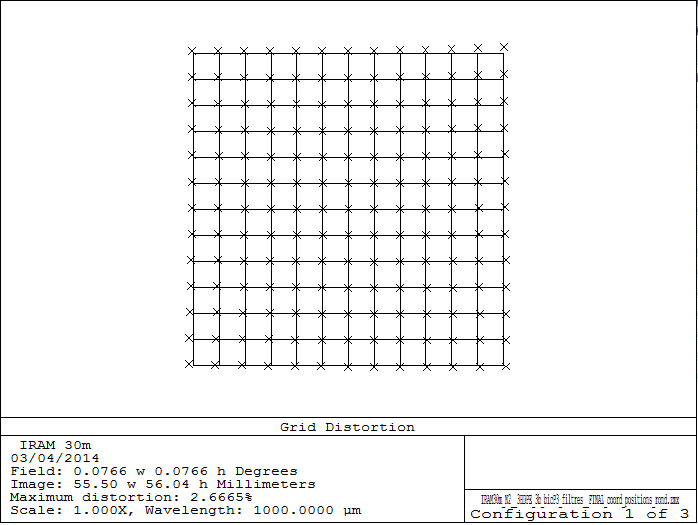
\includegraphics[width=0.9\textwidth]{Figures/NIKA2_Final_grid.png}
\caption{NIKA2 grid diagram simulated using ZEMAX. Crosses indicate
  the real coordinates on the Nasmyth image plan. {\bf question a
    Samuel: pourquoi les dimensions indiquees sont environs 4.5 arcmin
  de cote (et pas 6.5)?}}
 \label{fig:fov_grid_distortion_zemax}
\end{center}
\end{figure}

Figure \ref{fig:fov_grid_distortion_zemax} show the ZEMAX grid diagram for
NIKA2 simulated optic system. The maximum grid distortion is expected
to be of $2.7\%$ in NIKA2 $6.5'$ FOV. The distortion is the most
noticeable in the upper right corner of the Nasmyth plan, which is
also the area of the largest defocus w.r.t. to the center. 

An expected distortion of $2.7\%$ is at most a 5 arcsecond shift from the
center to the outside of the array.  The quoted measured distortions are not
too dissimilar once the different fitting methods have been taken into
account.

% FXD: this would need to be more ascertained. Lack of time to go further.
